%% beamer/knitr slides 
%% for Statistical Modeling and Data Visualization course @ UMass
%% Nicholas Reich: nick [at] schoolph.umass.edu


\documentclass[table]{beamer}\usepackage[]{graphicx}\usepackage[]{color}
% maxwidth is the original width if it is less than linewidth
% otherwise use linewidth (to make sure the graphics do not exceed the margin)
\makeatletter
\def\maxwidth{ %
  \ifdim\Gin@nat@width>\linewidth
    \linewidth
  \else
    \Gin@nat@width
  \fi
}
\makeatother

\definecolor{fgcolor}{rgb}{0.345, 0.345, 0.345}
\newcommand{\hlnum}[1]{\textcolor[rgb]{0.686,0.059,0.569}{#1}}%
\newcommand{\hlstr}[1]{\textcolor[rgb]{0.192,0.494,0.8}{#1}}%
\newcommand{\hlcom}[1]{\textcolor[rgb]{0.678,0.584,0.686}{\textit{#1}}}%
\newcommand{\hlopt}[1]{\textcolor[rgb]{0,0,0}{#1}}%
\newcommand{\hlstd}[1]{\textcolor[rgb]{0.345,0.345,0.345}{#1}}%
\newcommand{\hlkwa}[1]{\textcolor[rgb]{0.161,0.373,0.58}{\textbf{#1}}}%
\newcommand{\hlkwb}[1]{\textcolor[rgb]{0.69,0.353,0.396}{#1}}%
\newcommand{\hlkwc}[1]{\textcolor[rgb]{0.333,0.667,0.333}{#1}}%
\newcommand{\hlkwd}[1]{\textcolor[rgb]{0.737,0.353,0.396}{\textbf{#1}}}%
\let\hlipl\hlkwb

\usepackage{framed}
\makeatletter
\newenvironment{kframe}{%
 \def\at@end@of@kframe{}%
 \ifinner\ifhmode%
  \def\at@end@of@kframe{\end{minipage}}%
  \begin{minipage}{\columnwidth}%
 \fi\fi%
 \def\FrameCommand##1{\hskip\@totalleftmargin \hskip-\fboxsep
 \colorbox{shadecolor}{##1}\hskip-\fboxsep
     % There is no \\@totalrightmargin, so:
     \hskip-\linewidth \hskip-\@totalleftmargin \hskip\columnwidth}%
 \MakeFramed {\advance\hsize-\width
   \@totalleftmargin\z@ \linewidth\hsize
   \@setminipage}}%
 {\par\unskip\endMakeFramed%
 \at@end@of@kframe}
\makeatother

\definecolor{shadecolor}{rgb}{.97, .97, .97}
\definecolor{messagecolor}{rgb}{0, 0, 0}
\definecolor{warningcolor}{rgb}{1, 0, 1}
\definecolor{errorcolor}{rgb}{1, 0, 0}
\newenvironment{knitrout}{}{} % an empty environment to be redefined in TeX

\usepackage{alltt}


%       ************************************************
%       **        LaTeX preamble to be used with all 
%	**        statsTeachR labs/handouts.
%
%	Author: Nicholas G Reich
%	Last modified: 14 January 2014
%	************************************************

% \documentclass[table]{beamer}

%	Set theme (a nice plain one)
\usetheme{Malmoe}

%	Use named colors, set main color of theme
%		to match Web site color:
\definecolor{MainColor}{RGB}{10, 74, 109}
\colorlet{MainColorMedium}{MainColor!50}
\colorlet{MainColorLight}{MainColor!20}
\usecolortheme[named=MainColor]{structure} 

%	For tables
%[dvipsnames] [table]
\usepackage{xcolor}

%% calling tabu.sty, assuming a particular directory structure
\usepackage{../../slide-includes/tabu}	% Even fancier than tabulary
\usepackage{multirow}

%	Just for the degree symbol
\usepackage{textcomp}

%	Get rid of footline (page, author, etc. on each slide)
\setbeamertemplate{footline}{}
%	Get rid of navigation buttons
\setbeamertemplate{navigation symbols}{}

%	Make footnotes not ugly
\usepackage{hanging}
\setbeamertemplate{footnote}{\raggedright\hangpara{1em}{1}\makebox[1em][l]{\insertfootnotemark}\footnotesize\insertfootnotetext\par}

%	Text style for code snippets inline in text:
\newcommand{\codeInline}[1]{\texttt{#1}}

%	Text style for emphasis stronger than \emph:
%		(Note, this doesn't toggle the way \emph does.
%			(Note, this can be done, didn't seem worth the trouble.))
\newcommand{\strong}[1]{{\bfseries{#1}}}


%        ******	Define title page	**********************
\setbeamertemplate{title page}{
	{\color{MainColor}
	% There must be a better way than this -vspace at
	%	 the top and bottom of the page to reduce the 
	%	 bottom margin, but I can't find one that works.
	\vspace{-6em}

% 	% Go to a lot of trouble to get the title in a
% 	%	nice box, since customizing a beamer block
% 	%	does not entirely work here (I don't know why)
	\newlength{\titleBoxWidth}
	\setlength{\titleBoxWidth}{\textwidth}
	\addtolength{\titleBoxWidth}{-2.0em}
	\setlength{\fboxsep}{1.0em}
	\setlength{\fboxrule}{0pt}
	\fcolorbox{MainColor!25}{MainColor!25}{
		\parbox{\titleBoxWidth}{
			\raggedright
			\LARGE\textbf{\inserttitle}
		}	% end parbox
	}	% end fcolorbox

	\vfill
	\small{Author: \insertauthor}
	\vspace{\baselineskip}

	\small{\Course}

	\small{\Instructor}
	\vspace{\baselineskip}

	%\small{\emph{This material is part of the \strong{statsTeachR} project}}

	\vspace{0.33\baselineskip}\scriptsize{\emph{\LicenseText}}


		\vspace{-15em}

	}	% end color
	\clearpage
}	% end define title page

%        The following variables are assumed by the standard preamble:
%        Global variable containing module name:

\title{The language of modeling}
%	Global variable containing module shortname:
%		(Currently unused, may be used in future.)
\newcommand{\ModuleShortname}{modeling}
%	Global variable containing author name:
\author{Nicholas G Reich}
%	Global variable containing text of license terms:
\newcommand{\LicenseText}{Made available under the Creative Commons Attribution-ShareAlike 3.0 Unported License: http://creativecommons.org/licenses/by-sa/3.0/deed.en\textunderscore US }
%	Instructor: optional, can leave blank.
%		Recommended format: {Instructor: Jane Doe}
\newcommand{\Instructor}{}
%	Course: optional, can leave blank.
%		Recommended format: {Course: Biostatistics 101}
\newcommand{\Course}{}


\input{../../slide-includes/shortcuts}
\usepackage{bbm}

\hypersetup{colorlinks,linkcolor=,urlcolor=MainColor}


%	******	Document body begins here	**********************
\IfFileExists{upquote.sty}{\usepackage{upquote}}{}
\begin{document}

%	Title page
\begin{frame}[plain]
	\titlepage
\end{frame}

%	******	Everything through the above line must be placed at
%		the top of any TeX file using the statsTeachR standard
%		beamer preamble. 





%%%%%%%%%%%%%%%%%%%%%%%%%%%%%%%%%%%%%%%%%%


%%%%%%%%%%%%%%%%%%%%%%%%%%%%%%%%%%%%%%%%%%



\begin{frame}{Today's topics}

\bi
    \myitem The language of models
    \myitem Model formulas and coefficients 
\ei

\bigskip

{\bf Example:} predicting respiratory disease severity (``lung'' dataset)

\bigskip

{\bf Reading:} Kaplan, Chapters 4, 6-10.


\end{frame}

%%%%%%%%%%%%%%%%%%%%%%%%%%%%%%%%%%%%%%%%%%

\begin{frame}%{Warm up}

 Watch the first five minutes of \href{https://channel9.msdn.com/Events/useR-international-R-User-conference/useR2016/Towards-a-grammar-of-interactive-graphics}{Hadley Wickham's UseR! 2016 talk}

\vspace{1cm} 

\centering
\em
%  - models are fundamentally computational, the computer does it for you and that means that they scale
  `` ... every model has to make assumptions, and a model by its very nature cannot question those assumptions...

\vspace{1cm} 
  
 models can never fundamentally surprise you because they cannot question their own assumptions.'' %, but they do scale.'''


\end{frame}

%%%%%%%%%%%%%%%%%%%%%%%%%%%%%%%%%%%%%%%%%%

\begin{frame}{Statistical modeling}

The process of using data to describe the relationship between outcomes and predictors is called modeling.
\bi
  \myitem Models are models, not reality.
  \myitem ``All models are wrong, but some are useful." 
  \myitem Introduce structure to our model that balances realism with ``goodness of fit''. 
\ei

\end{frame}


%%%%%%%%%%%%%%%%%%%%%%%%%%%%%%%%%%%%%%%%%%

\begin{frame}[fragile]{Models are functions}

Definition: ``a {\bf function} is a relation between a set of inputs and a set of permissible outputs with the property that each input is related to exactly one output''.\footnote{Wikipedia, \href{https://en.wikipedia.org/wiki/Function_(mathematics)}{https://en.wikipedia.org/wiki/Function\_(mathematics)}}

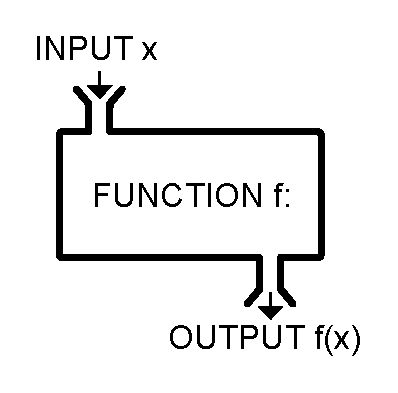
\includegraphics[width=.5\textwidth]{figure-static/Function_machine2}  

In statistical models, inputs are explanatory variables and outputs are ``typical'' or ``expected'' values of response variables. %There is always residual variation. The key challenge is judging whether the structure of a particular model is supported by evidence in the data.



\end{frame}


%%%%%%%%%%%%%%%%%%%%%%%%%%%%%%%%%%%%%%%%%%

\begin{frame}[fragile]{Models are functions: response variable}

Definition: ``a {\bf function} is a relation between a set of inputs and a set of permissible outputs with the property that each input is related to exactly one output''.\footnote{Wikipedia, \href{https://en.wikipedia.org/wiki/Function_(mathematics)}{https://en.wikipedia.org/wiki/Function\_(mathematics)}}

\vspace{2em}



We might write generally $$ y = f(x)$$ where $x$ could be a single variable or multiple variables.

\vspace{1em}

\bi
  \myitem {\bf The response variable} is $y$ the variable whose behavior or variation you are trying to understand. We might also call this the {\bf outcome variable}.
\ei

\end{frame}


%%%%%%%%%%%%%%%%%%%%%%%%%%%%%%%%%%%%%%%%%%

\begin{frame}{A common modeling tool: regression}

\bi
        \myitem The goal is to learn about the relationship between ``explanatory'' (or ``predictor'') variables of interest and a ``response`` (or  ``outcome'') of interest.
	\bi
		\myitem Some models focus on prediction.
		\myitem Other models focus on description.
	\ei
	\myitem Regression is an exercise in inferential statistics: we are drawing evidence and conclusions from data about ``complex aspects of reality'', i.e. ``noisy'' systems.
\ei


\end{frame}


%%%%%%%%%%%%%%%%%%%%%%%%%%%%%%%%%%%%%%%%%%


\begin{frame}[t]{Lung data example}

99 observations on patients who have sought treatment for the relief of respiratory disease symptoms. 

The variables are:
\bi
    \myitem {\tt disease} measure of disease severity (larger values indicates more serious condition).
    \myitem {\tt education} highest grade completed
    \myitem {\tt crowding} measure of crowding of living quarters (larger values indicate more crowding)
    \myitem {\tt airqual} measure of air quality at place of residence (larger number indicates poorer quality)
    \myitem {\tt nutrition} nutritional status (larger number indicates better nutrition)
    \myitem {\tt smoking} smoking status (1 if smoker, 0 if non-smoker)
\ei

What is the natural response variable here? Which variable are we trying to understand or explain?

\end{frame}


%%%%%%%%%%%%%%%%%%%%%%%%%%%%%%%%%%%%%%%%%%

\begin{frame}[fragile]{Lung data example: looking at variability in the response}



What variables will explain variation in disease severity?

\begin{knitrout}\footnotesize
\definecolor{shadecolor}{rgb}{0.969, 0.969, 0.969}\color{fgcolor}\begin{kframe}
\begin{alltt}
\hlstd{dat} \hlkwb{<-} \hlkwd{read.table}\hlstd{(}\hlstr{"../../data/lungc.txt"}\hlstd{,} \hlkwc{header}\hlstd{=}\hlnum{TRUE}\hlstd{)}
\hlkwd{ggplot}\hlstd{(dat,} \hlkwd{aes}\hlstd{(}\hlkwc{x}\hlstd{=disease))} \hlopt{+}
  \hlkwd{geom_histogram}\hlstd{()}
\end{alltt}
\end{kframe}
\includegraphics[width=\maxwidth]{figure/lung-plot-1-1} 

\end{knitrout}


\end{frame}


%%%%%%%%%%%%%%%%%%%%%%%%%%%%%%%%%%%%%%%%%%

\begin{frame}[fragile]{Models are functions: explanatory variables}

We might write generally $$ y = f(x)$$ where $x$ could be a single variable or multiple variables.

\bi
  \myitem {\bf The response variable} is $y$ the variable whose behavior or variation you are trying to understand. 
  \myitem {\bf The explanatory variables} $x$ are the variable(s) that you want to use to explain the variation in the response variable.
\ei

\end{frame}

%%%%%%%%%%%%%%%%%%%%%%%%%%%%%%%%%%%%%%%%%%

\begin{frame}[fragile]{Lung data example: explaining variability in the response}

Does crowding of living quarters explain some of the variation in disease severity?


\begin{knitrout}\footnotesize
\definecolor{shadecolor}{rgb}{0.969, 0.969, 0.969}\color{fgcolor}\begin{kframe}
\begin{alltt}
\hlkwd{ggplot}\hlstd{(dat,} \hlkwd{aes}\hlstd{(crowding, disease))} \hlopt{+}
  \hlkwd{geom_point}\hlstd{()}
\end{alltt}
\end{kframe}
\includegraphics[width=\maxwidth]{figure/lung-plots-1} 

\end{knitrout}


\end{frame}

%%%%%%%%%%%%%%%%%%%%%%%%%%%%%%%%%%%%%%%%%%

\begin{frame}[fragile]{Lung Data Example: explaining variability in the response}

Does smoking status explain some of the variation in disease severity?

\begin{knitrout}\footnotesize
\definecolor{shadecolor}{rgb}{0.969, 0.969, 0.969}\color{fgcolor}\begin{kframe}
\begin{alltt}
\hlkwd{ggplot}\hlstd{(dat,} \hlkwd{aes}\hlstd{(}\hlkwd{factor}\hlstd{(smoking), disease))} \hlopt{+} \hlkwd{geom_boxplot}\hlstd{()}
\end{alltt}
\end{kframe}
\includegraphics[width=\maxwidth]{figure/lung-plots-fac-smoke-1} 

\end{knitrout}


\end{frame}

%%%%%%%%%%%%%%%%%%%%%%%%%%%%%%%%%%%%%%%%%%

\begin{frame}[fragile]{Modeling recap}

We might write generally $$ y = f(x) $$ where $x$ could be a single variable or multiple variables.

\begin{block}{What will the "structure" of the model look like?}

\bi
  \myitem Most models we talk about will be a form of {\bf linear models}, e.g. $$ y = f(x) = \beta_0 + \beta_1 \cdot x $$.
  \myitem You must make a choice about {\bf model terms}. What does the right hand side of the above equation look like?
\ei

\end{block}

\end{frame}

%%%%%%%%%%%%%%%%%%%%%%%%%%%%%%%%%%%%%%%%%%

\begin{frame}[fragile]{Model terms: the intercept}

The intercept is a ``baseline`` that is included in nearly every model. What would your guess of disease severity be in the absence of any other information? $$y = \beta_0 $$

\begin{knitrout}\footnotesize
\definecolor{shadecolor}{rgb}{0.969, 0.969, 0.969}\color{fgcolor}\begin{kframe}
\begin{alltt}
\hlkwd{ggplot}\hlstd{(dat,} \hlkwd{aes}\hlstd{(}\hlkwc{y}\hlstd{=disease))} \hlopt{+}
  \hlkwd{geom_histogram}\hlstd{()} \hlopt{+} \hlkwd{geom_hline}\hlstd{(}\hlkwc{yintercept} \hlstd{=} \hlkwd{mean}\hlstd{(dat}\hlopt{$}\hlstd{disease),} \hlkwc{linetype}\hlstd{=}\hlnum{2}\hlstd{)}
\end{alltt}
\end{kframe}
\includegraphics[width=\maxwidth]{figure/lung-plot-intercept-1} 

\end{knitrout}

\end{frame}

%%%%%%%%%%%%%%%%%%%%%%%%%%%%%%%%%%%%%%%%%%

\begin{frame}[fragile]{Model terms: main terms}

Main terms model the effect of explanatory variables directly. $$y = \beta_0 + \beta_1 \cdot crowding $$

\begin{knitrout}\footnotesize
\definecolor{shadecolor}{rgb}{0.969, 0.969, 0.969}\color{fgcolor}\begin{kframe}
\begin{alltt}
\hlkwd{ggplot}\hlstd{(dat,} \hlkwd{aes}\hlstd{(crowding, disease))} \hlopt{+} \hlkwd{geom_point}\hlstd{()} \hlopt{+}
  \hlkwd{geom_smooth}\hlstd{(}\hlkwc{method}\hlstd{=}\hlstr{"lm"}\hlstd{,} \hlkwc{se}\hlstd{=}\hlnum{FALSE}\hlstd{)}
\end{alltt}
\end{kframe}
\includegraphics[width=\maxwidth]{figure/lung-plot-main-term-crowding-1} 

\end{knitrout}

\end{frame}

%%%%%%%%%%%%%%%%%%%%%%%%%%%%%%%%%%%%%%%%%%

\begin{frame}[fragile]{Model terms: main terms}

Main terms model the effect of explanatory variables directly. $$y = \beta_0 + \beta_2 \cdot smoking$$

\begin{knitrout}\footnotesize
\definecolor{shadecolor}{rgb}{0.969, 0.969, 0.969}\color{fgcolor}\begin{kframe}
\begin{alltt}
\hlkwd{ggplot}\hlstd{(dat,} \hlkwd{aes}\hlstd{(}\hlkwc{x}\hlstd{=}\hlkwd{factor}\hlstd{(smoking),} \hlkwc{y}\hlstd{=disease))} \hlopt{+}
  \hlkwd{geom_boxplot}\hlstd{()}
\end{alltt}
\end{kframe}
\includegraphics[width=\maxwidth]{figure/lung-plot-main-term-smoking-1} 

\end{knitrout}

\end{frame}

%%%%%%%%%%%%%%%%%%%%%%%%%%%%%%%%%%%%%%%%%%

\begin{frame}[fragile]{Model terms: interaction terms}

Interaction terms allow for different explanatory variables to modulate the relationship of each other to the response variable. $$y = \beta_0 + \beta_1 \cdot crowding + \beta_2 \cdot smoking + \beta_3 \cdot crowding \cdot smoking$$

\begin{knitrout}\footnotesize
\definecolor{shadecolor}{rgb}{0.969, 0.969, 0.969}\color{fgcolor}\begin{kframe}
\begin{alltt}
\hlkwd{ggplot}\hlstd{(dat,} \hlkwd{aes}\hlstd{(crowding, disease,} \hlkwc{color}\hlstd{=}\hlkwd{factor}\hlstd{(smoking)))} \hlopt{+}
  \hlkwd{geom_point}\hlstd{()} \hlopt{+} \hlkwd{geom_smooth}\hlstd{(}\hlkwc{method}\hlstd{=}\hlstr{"lm"}\hlstd{,} \hlkwc{se}\hlstd{=}\hlnum{FALSE}\hlstd{)}
\end{alltt}
\end{kframe}
\includegraphics[width=\maxwidth]{figure/lung-plot-interaction-1} 

\end{knitrout}

\end{frame}


%%%%%%%%%%%%%%%%%%%%%%%%%%%%%%%%%%%%%%%%%%

\begin{frame}[fragile]{Model terms: recap}

\bi
  \myitem {\bf The intercept} is a ``baseline`` that is included in nearly every model. What would your guess of disease severity be in the absence of any other information?
  \myitem {\bf Main terms} model the effect of explanatory variables directly.
  \myitem {\bf Interaction terms} allow for different explanatory variables to modulate the relationship of each other to the response variable.
  \myitem {\bf Smooth terms} and {\bf transformation terms}: to come soon!
\ei

\end{frame}


\end{document}
